\documentclass[sigconf, nonacm]{acmart}

\usepackage{natbib}
\usepackage{quoting}
\usepackage{amsmath}

%%
%% \BibTeX command to typeset BibTeX logo in the docs
\AtBeginDocument{%
  \providecommand\BibTeX{{%
    Bib\TeX}}}



%% These commands are for a PROCEEDINGS abstract or paper.
\acmConference[Explainable and Trustworthy AI - Project]{}{}{}



\begin{document}

\title{P3 - Exploring linear equations as means for a more interpretable decision with Deep Concept Reasoning}


%%
%% The "author" 
\author{Ewen Rondel}
\affiliation{%
  \text{s321468}
  \\
  \institution{Politecnico di Torino}
  \city{Turin}
  \country{Italy}
}

\author{João Almeida}
\affiliation{%
  \text{s332204}
  \\
  \institution{Politecnico di Torino}
  \city{Turin}
  \country{Italy}
}
\author{Thomas Lepretre}
\affiliation{%
  \text{s332585}
  \\
  \institution{Politecnico di Torino}
  \city{Turin}
  \country{Italy}
}



%%
\begin{abstract}
\vspace{2pt}
After exploring different ideas for enhancing the interpretability of concept-based models, we propose a novel variant of the Deep Concept Reasoning (DCR) \cite{barbiero2023interpretable} model, focusing on utilizing linear equations to achieve interpretable predictions. The traditional Concept Embedding Model (CEM) \cite{espinosa2022concept} offers robust generalization capabilities akin to black-box models, but lacks interpretability due to its high-dimensional concept embeddings. Conversely, the DCR model provides interpretable predictions by generating logic rules over concept embeddings, yet its interpretability paradigm can be restrictive and its accuracy is slightly affected because of it.

Our approach aims to simplify and enhance the accuracy of the DCR model by employing linear equations over concept embeddings. This modification maintains the end-to-end trainability and augment the accuracy of the DCR, while offering a more straightforward and globally interpretable prediction mechanism. Reviewing the previous work on supervised concept-based models, we emphasize the methodologies and limitations of the CEM and the DCR.

The proposed model is implemented and rigorously tested on both synthetic and real-world datasets. We evaluate its performance against standard DCR using various metrics, focusing on generalization capability and interpretability. Preliminary results indicate that our model not only retains a certain interpretability of the DCR but also improves the task accuracy, making it a promising tool for applications requiring effective transparent decision-making processes.
\end{abstract}



%% OPTIONAL 
%% Keywords. The author(s) should pick words that accurately describe the work being presented. Separate the keywords with commas.
\keywords{}



%%
%% This command processes the author and affiliation and title information and builds the first part of the formatted document.
\maketitle

\section{Introduction}
\vspace{2pt}
In recent years, the field of Explainable Artificial Intelligence (XAI) has gained significant attention as machine learning models become increasingly complex and ubiquitous in decision-making processes. While these advanced models offer impressive predictive capabilities, their lack of transparency often hinders their adoption in critical domains where interpretability is paramount. Concept-based models have emerged as a promising approach to bridge the gap between high performance and interpretability in machine learning.
The evolution of concept-based models has seen several key developments, from the Concept Bottleneck Model (CBM) \cite{koh2020concept} to the Concept Embedding Model (CEM) \cite{espinosa2022concept}, and most recently, the Deep Concept Reasoning (DCR) model \cite{barbiero2023interpretable}. Each iteration has aimed to improve upon its predecessors, balancing, and with the DCR, outright challenging, the trade-off between generalization capability and interpretability. However, further improvements in achieving clear, intuitive explanations for model decisions without sacrificing high performance can still be explored.
Our research focuses on developing a novel variant of the DCR model that maintains its end-to-end trainability and interpretability power while enhancing its task accuracy through the use of linear equations. This approach aims to simplify the interpretation of concept embeddings, providing a more accessible and globally interpretable prediction mechanism compared to the logic rules employed in the original DCR model.
The primary objectives of this study are to: \vspace{2pt}

\begin{enumerate}
    \item Analyze the strengths and limitations of existing supervised concept-based models, with a particular focus on the CEM and the DCR. \vspace{4pt}
    \item Propose and implement a new model that utilizes linear equations for interpretable predictions over concept embeddings. \vspace{8pt}
    \item Evaluate the performance and interpretability of our proposed model against the standard DCR model using both synthetic and real-world datasets. \vspace{2pt}
\end{enumerate}

With these objectives in mind, we aim to contribute to the ongoing development of explainable AI systems that can be reliably deployed in scenarios requiring both high performance and transparent decision-making processes, by further pushing the ease of interpretability of the models. \vspace{8pt}

\section{Related work}
\vspace{2pt}
The field of concept-based models in machine learning has seen rapid advancement in recent years, with each new model building upon the strengths of its predecessors while addressing their limitations. This section provides an overview of the key developments leading to our proposed model. \vspace{6pt}

\subsection{Concept Bottleneck Model (CBM)}
\vspace{2pt}
Koh et al. introduced the Concept Bottleneck Model in 2020 \cite{koh2020concept}, marking a significant step towards interpretable machine learning. The CBM structures the prediction process into two distinct stages: concept prediction and task prediction. By forcing the model to make predictions through an intermediate layer of human-specified concepts, the CBM provides a level of transparency to the decision-making process. However, the use of single neurons to represent concepts limits the model's representation capability, often resulting in a trade-off between interpretability and predictive performance. \vspace{6pt}

\subsection{Concept Embedding Model (CEM)}
\vspace{2pt}
To address the limitations of CBM, Zarlenga et al. proposed the Concept Embedding Model in 2022 \cite{espinosa2022concept}. The CEM represents concepts as embeddings rather than single neurons, significantly enhancing the model's representation capability. This approach allows the CEM to achieve generalization performance comparable to black-box end-to-end models while retaining the ability to interact with the model through concepts. However, the high-dimensional nature of concept embeddings in the CEM makes it challenging to interpret the model's decisions, as the individual dimensions of these embeddings lack clear semantic meaning. \vspace{6pt}

\subsection{Deep Concept Reasoning (DCR)}
\vspace{2pt}
Building upon the strengths of CEM, Barbiero et al. introduced the Deep Concept Reasoning model in 2023 \cite{barbiero2023interpretable}. The DCR is an end-to-end trainable model that provides interpretable predictions in the form of logic rules over concept embeddings. For each sample, DCR predicts a rule that holds true for the given sample's concept embeddings, which is then symbolically executed over the concept scores. This approach offers a novel way to interpret the model's decisions, bridging the gap between the high performance of concept embeddings and the interpretability desired in many applications. \vspace{8pt}

\section{Research gaps}
\vspace{2pt}
While the DCR model represents a significant advancement in interpretable concept-based models, some current limitations may offer opportunities for improvement. \vspace{6pt}

\subsection{Complexity of Logic Rules}
\vspace{2pt}
In situations where a large number of concepts are necessary to differentiate between tasks, the DCR may generate increasingly complex rules. Although this issue is not prevalent in most current benchmark datasets and real-world applications, it highlights a potential scalability concern for more intricate problem domains. Developing methods to manage rule complexity in high-dimensional concept spaces could enhance the model's applicability to a broader range of problems. \vspace{6pt}

\subsection{Global Interpretability}
\vspace{2pt}
A key limitation of the DCR is the potential misalignment between its global behavior and the rules it generates. This discrepancy can pose challenges in scenarios where a comprehensive understanding of the model's overall decision-making process is crucial. Enhancing the model's ability to provide accurate global interpretations without sacrificing local explanatory power remains an open challenge. \vspace{6pt}

\subsection{Dependency on Concept Embeddings}
\vspace{2pt}
The DCR's reliance on concept embeddings as inputs presupposes the availability of concept-based datasets or robust concept-discovery techniques. This dependency may limit the model's applicability in domains where such resources are scarce or where concept identification is particularly challenging. Exploring ways to integrate concept discovery within the DCR framework or developing methods to operate with less refined concept representations could broaden the model's usefulness. \vspace{6pt}

\subsection{Trade-off Between Expressiveness and Simplicity}
\vspace{2pt}
While logic rules offer high expressiveness, they may not always be the most concise or intuitive way to represent relationships between concepts and predictions. There's an opportunity to explore alternative representation methods that balance expressiveness with simplicity, potentially making the model's decisions more accessible to a wider audience.

By addressing these research gaps, particularly the complexity of logic rules, we aim to develop a variant of DCR that maintains its strengths in concept-based reasoning while offering more intuitive and widely accessible interpretations. Our proposed approach using linear equations seeks to tackle these challenges, especially in simplifying the interpretability mechanism without sacrificing the model's predictive power. \vspace{8pt}

\section{Methodology}
\vspace{2pt}
Our proposed variant of the Deep Concept Reasoning (DCR) model aims to enhance accuracy while maintaining the model's explanative power. We achieve this by replacing the complex fuzzy logic rules used in the original DCR with a more intuitive linear equation approach. \vspace{6pt}

\subsection{Model Architecture}
\vspace{2pt}
The core of our model remains similar to the original DCR, consisting of three main components: \vspace{4pt}
\begin{enumerate}
    \item Encoder: Encodes the input in some way, the architecture of this component will vary depending on the dataset and problem being handled.\vspace{8pt}
    \item Concept Embedding Layer: Creates the concept embeddings to be used by the DCR using the encoded input.\vspace{8pt}
    \item Concept Reasoning Layer: Creates a linear equation using the concepts detection as to generate a prediction from them.\vspace{8pt}
\end{enumerate}
The only modification in our approach lies in the Concept Reasoning Layer, which we have redesigned to use linear equations instead of fuzzy logic rules. \vspace{6pt}

\subsection{Linear Equation Concept Reasoning}
\vspace{2pt}
In our variant, the Concept Reasoning Layer implements a linear transformation of the concept embeddings to generate class predictions. This approach can be represented by the following equation:

\begin{equation}
    y = \sigma(Wx + b)
\end{equation}

Where:
\begin{itemize}
    \item $y$ is the vector of class predictions
    \item $\sigma$ is the sigmoid activation function
    \item $W$ is the weight matrix
    \item $x$ is the flattened concept embedding vector
    \item $b$ is the bias term \vspace{8pt}
\end{itemize}

This linear approach offers several advantages: \vspace{4pt}

\begin{enumerate}
    \item Simplicity: Linear equations can be more intuitive and easier to interpret than logic rules which can be complex depending on the domain.\vspace{8pt}
    \item Scalability: The linear model can handle a large number of concepts without exponentially increasing complexity.\vspace{8pt}
    \item Continuous representation: Unlike binary logic rules, linear equations can capture nuanced relationships between concepts and classes.
\end{enumerate} \vspace{6pt}

\subsection{Interpretability Mechanism}
\vspace{2pt}
Our model provides interpretable predictions through an analysis of the weights in the linear transformation. For each class, we can express the prediction as a weighted sum of concept contributions:

\begin{equation}
    \text{class\_score} = w_1 \cdot c_1 + w_2 \cdot c_2 + \ldots + w_n \cdot c_n
\end{equation}

Where $w_i$ represents the weight associated with concept $c_i$.

To enhance interpretability, we normalize these weights to show the relative importance of each concept in the decision-making process. For each class, we calculate:\vspace{8pt}

\begin{enumerate}
    \item The total absolute weight: $\sum_{i=1}^n |w_i|$ \vspace{8pt}
    \item The percentage contribution of each concept: $\frac{|w_i|}{\sum_{i=1}^n |w_i|} \cdot 100\%$ \vspace{8pt}
\end{enumerate}

This allows us to present explanations in the form of linear equations, where each term includes:
\begin{itemize}
    \item The weight of the concept
    \item The concept name
    \item The sign of the contribution (positive or negative)
    \item The percentage contribution to the overall decision
\end{itemize} \vspace{6pt}

\subsection{Global vs. Local Interpretability}
\vspace{2pt}
Unlike the original DCR, which focused on local interpretability through sample-specific logic rules, our approach naturally provides both local and global interpretability: \vspace{4pt}

\begin{enumerate}
    \item \textbf{Global Interpretability:} The linear transformation weights provide a clear and consistent explanation of the model's overall behavior for all samples. In particular, they make it easy to attest to the importance of each feature/concept in the decision-making process.\vspace{8pt}
    
    \item \textbf{Local Interpretability:} By combining the global weights with the specific concept embeddings or predictions for a given sample, we can generate sample-specific explanations.
\end{enumerate}

This dual approach to interpretability addresses one of the key limitations of the original DCR model. \vspace{6pt}

\subsection{Training and Optimization}
\vspace{2pt}
The training process for our model remains end-to-end, similar to the original DCR. We use backpropagation to optimize all components of the model simultaneously, including the concept encoder, concept predictor, and our modified concept reasoning layer.

The loss function combines: \vspace{4pt}
\begin{enumerate}
    \item A concept prediction loss (e.g., binary cross-entropy for each concept) \vspace{8pt}
    \item A classification loss for the final predictions \vspace{8pt}
\end{enumerate}

This ensures that the model learns meaningful concept representations while optimizing for the target task. \vspace{6pt}

\subsection{Summary}
\vspace{2pt}
In summary, our methodology preserves the concept-based approach of the DCR while simplifying the reasoning mechanism through linear equations. This modification aims to enhance task accuracy, scalability, and the balance between global and local explanations, addressing several of the research gaps identified in the original DCR model, while maintaining a good level of interpretability. \vspace{8pt}

\section{Experiments and analysis}
\vspace{2pt}
For analysing the capabilities and performance of our Linear DCR variant, we employed a series of tests across several datasets, both synthetic and taken from real-world data. To be able to draw some comparisons, we have tested these datasets with the original DCR model introduced by \citet{barbiero2023interpretable}, as to analyse the key differences between the model and our proposed variant. \vspace{6pt}

\begin{figure*}[ht]
\centering
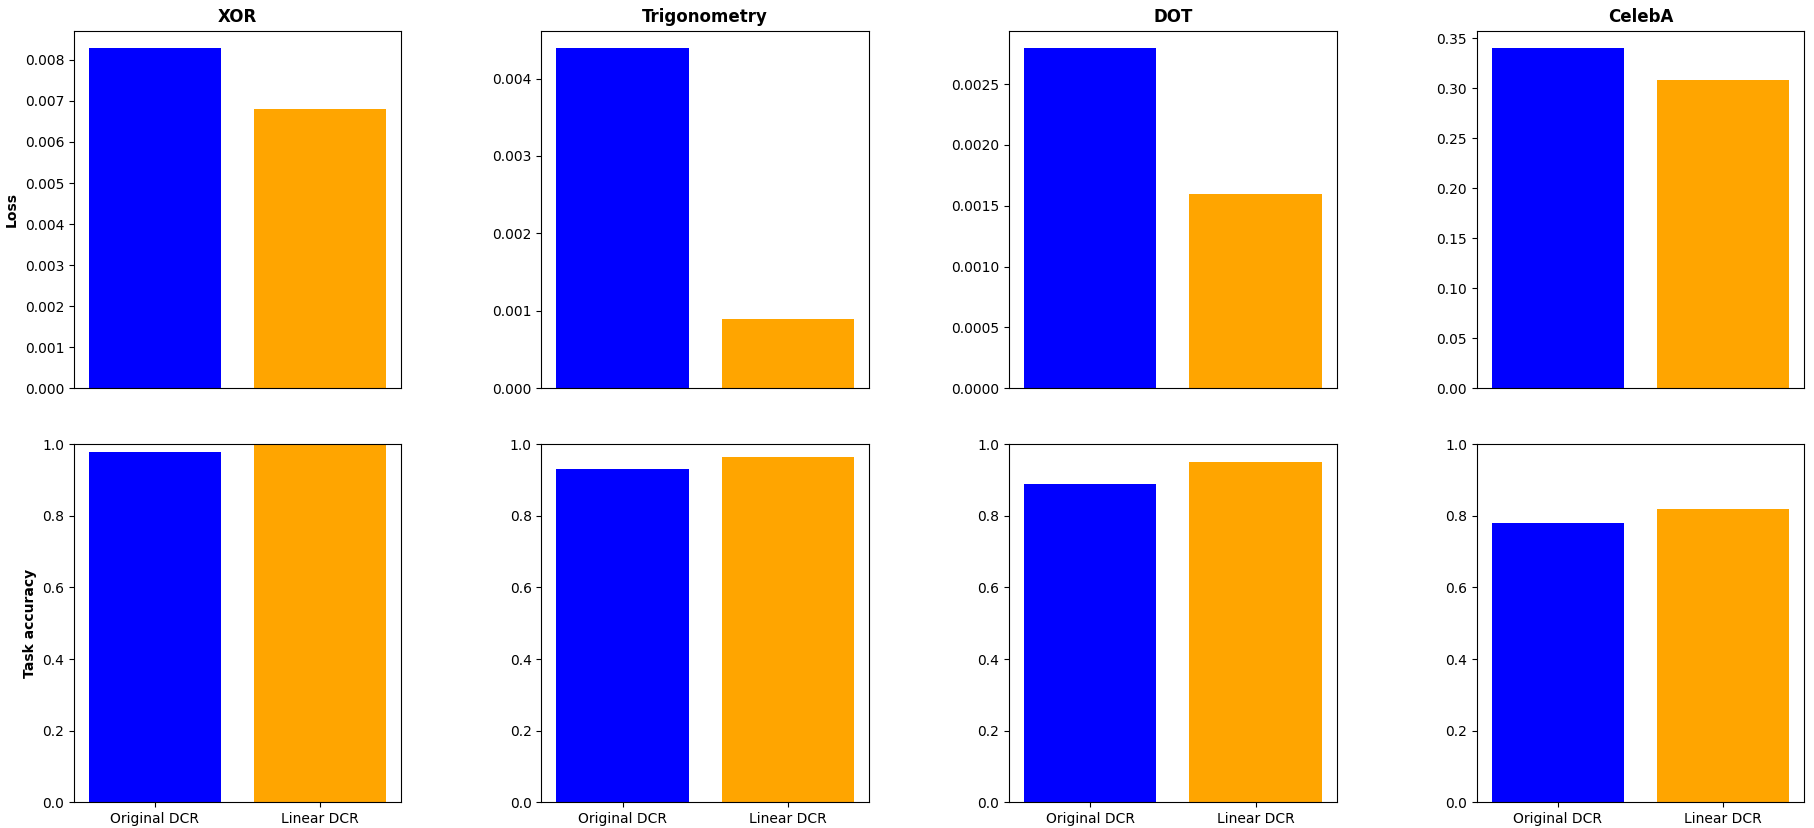
\includegraphics[width=1\linewidth]{./DCR_comparisons.png}
\caption{Metrics comparison between the original DCR and our linear variant across synthetic and real datasets}
\label{fig:figure1}
\end{figure*}

\subsection{Synthetic Datasets}
\vspace{2pt}
Inspired by the work of \citet{barbiero2023interpretable}, we use a very similar set of synthetic datasets. We have made an adjustment to the Trigonometry dataset in order to make its task more challenging, and give a bigger margin of improvement for our Linear DCR variant compared to the original model. \vspace{8pt}

\textbf{XOR} This dataset is built around the exclusive-OR (XOR) problem introduced by \citet{minsky1969perceptrons}. As described by \citet{barbiero2023interpretable}, the dataset is as follows:
\begin{quote}
"We draw input samples from a uniform distribution in the unit square \( x \in [0, 1]^2 \) and define two binary concepts \(\{c_1, c_2\}\) by using the Boolean (discrete) version of the input features \( c_i = \mathbb{1}_{x_i > 0.5} \). Finally, we construct a downstream task label using the XOR of the two concepts \( y = c_1 \oplus c_2 \)."
\end{quote} \vspace{8pt}

\textbf{Trigonometry} The second synthetic dataset was inspired by the toy dataset used by \citet{mahinpei2021promisespitfallsblackboxconcept}, as described in Appendix Section D of their paper. Our specific implementation is very similar to the one by \citet{barbiero2023interpretable}:
\begin{quote}
"We construct synthetic concept-annotated samples from three independent latent normal random variables \( h_i \sim \mathcal{N}(0, 2) \). Each of the 7 features in each sample is constructed via a non-invertible function transformation of the latent factors, where 3 features are of the form \( \sin(h_i) + h_i \), 3 features of the form \( \cos(h_i) + h_i \), and 1 is the nonlinear combination \( h_1^2 + h_2^2 + h_3^2 \). Each sample is then associated with 3 binary concepts representing the sign of their corresponding latent variables, i.e., \( c_i = (h_i > 0) \). In order to make this task Boolean-undecidable from its binary concepts, we modify the downstream task proposed by \citet{mahinpei2021promisespitfallsblackboxconcept} by assigning each sample a label \( y = \mathbb{1}_{(h_1 + h_2) > 0} \) indicating whether \( h_1 + h_2 \) is positive or not.
"
Our only adjustment has been to remove one of the three concepts, as to, as mentioned before, reduce the overall accuracy of the models and increase the room for improvement.
\end{quote} \vspace{8pt}

\textbf{Dot} The final synthetic dataset, the Dot dataset, or Vector dataset, is described by \citet{barbiero2023interpretable} as:
\begin{quote}
The Vector dataset is based on four 2-dimensional latent factors from which concepts and task labels are constructed. Two of these four vectors correspond to fixed reference vectors \( \mathbf{w}^+ \) and \( \mathbf{w}^- \), while the remaining two vectors \( \{ \mathbf{v}_i \}_{i=1}^2 \) are sampled from a 2-dimensional normal distribution. We then create four input features as the sum and difference of the two factors \( \mathbf{v}_i \). From this, we create two binary concepts representing whether or not the latent factors \( \mathbf{v}_i \) point in the same direction as the reference vectors \( \mathbf{w}_j \) (as determined by their dot products). Finally, we construct the downstream task as determining whether or not vectors \( \mathbf{v}_1 \) and \( \mathbf{v}_2 \) point in the same direction (as determined by their dot product).
\end{quote} \vspace{8pt}

\textbf{Concept Embedding} On all synthetic datasets, we employ, similarly to \citet{barbiero2023interpretable}, the Concept Embedding Model \citep{espinosa2022concept} implemented as an MLP with hidden layer sizes \{32, 32\} and LeakyReLU activations. We learn embeddings with \( m = 16 \) activations. \vspace{8pt}

\textbf{Hyperparameters} Across the synthetic datasets, each is generated with 1000 samples. We use a 67\%-33\% split for training and testing. The learning rate was set to 0.01, and we ran training for 501 epochs. \vspace{8pt}

\textbf{Task Accuracy} Across the three synthetic datasets, similar results can be seen. We can observe a small increment in task accuracy in all of them with our Linear DCR variant, with XOR going from 99.09\% with the original model to 100\% with our linear variant, Trigonometry going from 93.03\% to 96.06\% and Dot going from 89.70\% to 94.55\%.\\
However, with such high results, it was difficult to compare them with those of the previous DCR, as both were too efficient. We therefore needed to test the models on a more complicated dataset, representative of a real-life situation.\vspace{8pt}

\textbf{Loss} In addition to an improvement for the task accuracy, we also observe a significant improvement for the loss: -18\% for XOR, -80\% for Trigonometry and -43\% for Dot.\vspace{8pt}

\subsection{Real Dataset}
\vspace{2pt}
\textbf{CelebA} As a real-life dataset, we used CelebFaces Attributes Dataset (or CelebA), which is a large-scale face attributes dataset with more than 200K celebrity images, each with 40 attribute annotations. For computing resources reasons, we only used a subset of CelebA, with 20699 images. CelebA was one of the datasets used to evaluate the DCR, so it is suitable to use it to compare the DCR to our linear variant. Examples of face attribute annotations, or concepts, are "Eyeglasses", Wavy\textunderscore Hair", "Oval\textunderscore Face", or even "Mouth\textunderscore Slightly\textunderscore Open".

For the evaluated task in our experiment, we chose to predict if images represent a male or a female celebrity. This attribute is called "Male" and is set to either True or False.

To do so, we selected 3 concepts based on 2 factors: \vspace{4pt}
\begin{enumerate}
    \item Discrimination between Male and Female: Using a Student's t-test, we compared differences between means for every concepts. With this, we have obtained a list of the theoretically most useful concepts for differentiating males from females.\vspace{8pt}
    \item Concept Accuracy: The Concept Embedding Layer (using the Encoder's embeddings) had to have a high concept accuracy using them, so we know that they are well detected. It enabled us to refine the model by selecting concepts that were better recognized by it, rather than those that were better at discriminating but less well recognized.
\end{enumerate}
The 3 concepts that we chose are "Wearing\textunderscore Necktie", "Gray\textunderscore Hair" and "Bald". \vspace{8pt}

\textbf{Encoder} To feed our Encoder, prior to the Concept Embedding Layer, we needed to pre-process the images. The first thing we did was to use a shifted version of the CelebA dataset, so the celebrities were centered. And the second thing, in order to fit our computer resources limits, we resized the images into a 3x64x64 format, inspired by Espinosa Zarlenga et al. (2022) \cite{espinosa2022concept}.

Our Encoder is using a pre-trained ResNet architecture (He et al., 2016 \cite{he2016residuallearning}), replacing the last layer by a fully connected layer with \( m = 16 \) activations. But instead of using ResNet-34 like Espinosa Zarlenga et al. (2022) \cite{espinosa2022concept}, we use ResNet-18, taking advantage of its relative lightness. \vspace{8pt}

\textbf{Hyperparameters} If someone wants to reproduce the experiment with the same main hyperparameters, the train/test split has to be set to 80/20, the number of epochs has to be set to 50, and the learning rate has to be set to 0,01. \vspace{8pt}

\textbf{Concepts Accuracy} The concepts accuracy is the accuracy with which the Concept Embedding Layer detects the concepts in the input images. As both the original DCR and our Linear DCR variant use the same Concept Embedding Layer, the concept accuracy remains the same, which is about 89\%. \vspace{8pt}

\textbf{Task Accuracy} With our custom CelebA subset and our hyperparameters, the original DCR obtains an accuracy of about 78\% (on average, through multiple runs) in the task of predicting if a celebrity is a male or a female (see Figure 1). In comparison, our Linear DCR variant obtains a task accuracy of about 81\%. It represents a 3\% increase. And even if the gap between the results is still not gigantic, we can notice a slight improvement from an already well-performing model. \vspace{8pt}

\textbf{Loss} Regarding the overall loss (including concepts detection and task prediction), which is calculated the same way for both models, the original DCR's loss is about 0.345 on average (see Figure 1). In comparison, our Linear DCR variant's loss is about 0.300, which represents a 13\% decrease. This suggests that our Linear DCR variant is potentially more confident in its predictions, and is potentially able to generalize slightly better on new unseen data.  \vspace{8pt}


\section{Conclusions}
\vspace{2pt}
Through this study, we have achieved several of our objectives, which can be summarized as a functional and high-performance implementation of a linear version of a Concept Reasoning Layer.

This translates into a more interpretable model, thanks to its linear format, which allows us to better grasp the importance of each concept in the classification.

In addition, we obtained slightly better results than the ancient DCR, especially when used on the CelebA dataset.

The limitations of our study probably lie in the lack of variety in our tests. Indeed, apart from syntetic datasets, we only have one experiment that could be adapted to a real situation. One possible direction of research would therefore be to create other datasets to test different types of model, so as to be able to compare DCR-type models more easily. 

Another line of progress would be to find an even more powerful version of DCR, to perhaps approach the results that can be achieved with non-interpretable models.
\vspace{8pt}


%%
%% The next two lines define the bibliography style to be used, and
%% the bibliography file.
\bibliographystyle{ACM-Reference-Format}
\bibliography{biblio}


\end{document}
\endinput
%%